\begin{frame}{Rogue AP – Drill Order}
	\framesubtitle{Controlled Wi-Fi Scenario}

	\begin{columns}[T,onlytextwidth]



		% -------- Rechte Spalte: Bild --------
		\column{0.60\textwidth}
		\centering
		\includegraphics[width=0.7\linewidth]{assets/rogue-ap}
			% -------- Linke Spalte: Drill Timeline --------
		\column{0.9\textwidth}

		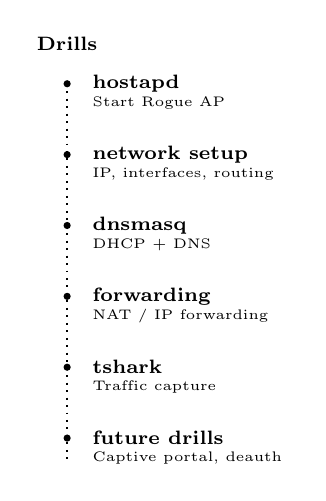
\begin{tikzpicture}[transform shape]
			\node[anchor=south] at (0,0.3) {\scriptsize\textbf{Drills}};

			% Linie
			\draw[dotted, line width=0.7pt] (0,0) -- (0,-4.8);

			% Punkte + Labels
			\foreach \y/\title/\desc in {
				0/{hostapd}/{Start Rogue AP},
				-0.9/{network setup}/{IP, interfaces, routing},
				-1.8/{dnsmasq}/{DHCP + DNS},
				-2.7/{forwarding}/{NAT / IP forwarding},
				-3.6/{tshark}/{Traffic capture},
				-4.5/{future drills}/{Captive portal, deauth}
			}{
				\fill (0,\y) circle (1.3pt);
				\node[anchor=west] at (0.20,\y) {\scriptsize\textbf{\title}};
				\node[anchor=west, align=left] at (0.20,\y-0.25) {\tiny \desc};
			}
		\end{tikzpicture}

	\end{columns}
\end{frame}
